\section{空间直线、平面的平行}

本节要点:
\begin{itemize}
    \item 掌握线面平行的定义;
    \item 掌握线面平行的定理;
    \item 掌握线面平行的性质。
\end{itemize}

~

直线和平面、平面和平面的关系中,重点是平行和垂直关系,本节讨论平行,依照“定义—定理—性质”的步骤理解本节内容。

线面平行:
\begin{itemize}
    \item 定义:直线和平面没有交点;
    \item 定理:若直线和平面内一条直线平行,则线面平行,如下左图;
    \item 性质:若线面平行,则直线和交线平行,如下右图。
\end{itemize}

\begin{figure}[h]
\centering
\begin{minipage}{.49\textwidth}
\centering
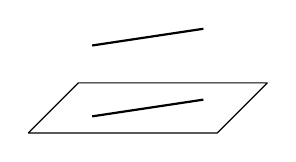
\begin{tikzpicture}[style={x={(-135:0.5)},y={(1cm,0)},z={(0,1cm)}}, line join=round, scale=0.3]
\draw (3,-4,0)--(3,4,0)--(-3,4,0)--(-3,-4,0)--(3,-4,0);
\draw[thick] (1,-2,0)--(-1,2,0) (1,-2,3)--(-1,2,3);
\end{tikzpicture}
\end{minipage}
\begin{minipage}{.49\textwidth}
\centering
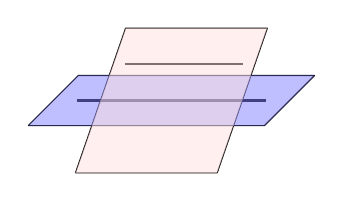
\begin{tikzpicture}[style={x={(-135:0.5)},y={(1cm,0)},z={(0,1cm)}}, line join=round, scale=0.3]
\draw (3,-5,0)--(3,5,0)--(-3,5,0)--(-3,-5,0)--(3,-5,0);
\draw (3,-3,-2)--(3,3,-2)--(-3,3,2)--(-3,-3,2)--(3,-3,-2);
\draw[thick] (0,-4,0)--(0,4,0) (-1.5,-2.5,1)--(-1.5,2.5,1);
\fill[blue!50!white,opacity=0.5] (3,-5,0)--(3,5,0)--(-3,5,0)--(-3,-5,0)--cycle;
\fill[pink!50!white,opacity=0.5] (3,-3,-2)--(3,3,-2)--(-3,3,2)--(-3,-3,2)--cycle;
\end{tikzpicture}
\end{minipage}
\end{figure}

\begin{tcolorbox}
教材对定义和定理讨论较少,倒是对性质给出了证明,反复阅读性质的证明过程P137,领会精神!
\end{tcolorbox}

面面平行:
\begin{itemize}
    \item 定义:平面和平面没有交点;
    \item 定理:若平面内两相交直线和平面平行,则面面平行,如下左图;
    \item 性质:若面面平行,则第三平面产生的两条交线平行,如下右图。
\end{itemize}

\begin{figure}[h]
\centering
\begin{minipage}{.49\textwidth}
\centering
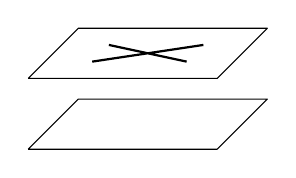
\begin{tikzpicture}[style={x={(-135:0.5)},y={(1cm,0)},z={(0,1cm)}}, line join=round, scale=0.3]
\draw (3,-4,0)--(3,4,0)--(-3,4,0)--(-3,-4,0)--(3,-4,0);
\draw (3,-4,-3)--(3,4,-3)--(-3,4,-3)--(-3,-4,-3)--(3,-4,-3);
\draw[thick] (1,-2,0)--(-1,2,0) (-1,-2,0)--(1,2,0);
\end{tikzpicture}
\end{minipage}
\begin{minipage}{.49\textwidth}
\centering
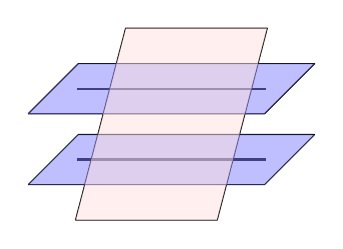
\begin{tikzpicture}[style={x={(-135:0.5)},y={(1cm,0)},z={(0,1cm)}}, line join=round, scale=0.3]
\draw (3,-5,1.5)--(3,5,1.5)--(-3,5,1.5)--(-3,-5,1.5)--(3,-5,1.5);
\draw (3,-5,-1.5)--(3,5,-1.5)--(-3,5,-1.5)--(-3,-5,-1.5)--(3,-5,-1.5);
\draw (3,-3,-3)--(3,3,-3)--(-3,3,3)--(-3,-3,3)--(3,-3,-3);
\draw[thick] (0,-4,1.5)--(0,4,1.5) (0,-4,-1.5)--(0,4,-1.5);
\fill[blue!50!white,opacity=0.5] (3,-5,1.5)--(3,5,1.5)--(-3,5,1.5)--(-3,-5,1.5)--cycle;
\fill[blue!50!white,opacity=0.5] (3,-5,-1.5)--(3,5,-1.5)--(-3,5,-1.5)--(-3,-5,-1.5)--cycle;
\fill[pink!50!white,opacity=0.5] (3,-3,-3)--(3,3,-3)--(-3,3,3)--(-3,-3,3)--cycle;
\end{tikzpicture}
\end{minipage}
\end{figure}

\begin{tcolorbox}
同样,教材对定义和定理讨论较少,对性质的证明过程需要反复阅读P141,领会精神!
\end{tcolorbox}

定义很简单,还没法用于判断,定理用于判断,也称为判断定理。所以解题思路就是先用定理判定平行,然后用性质得出需要的结论。




